%!TEX root = ../main.tex
%%%%%%%%%%%%%%%%%%%%%%%%%%%%%%%%%%
% Links:
%
% Difficulty:
% Companies: 
%%%%%%%%%%%%%%%%%%%%%%%%%%%%%%%%%%


%\begin{figure}
%	\centering
%	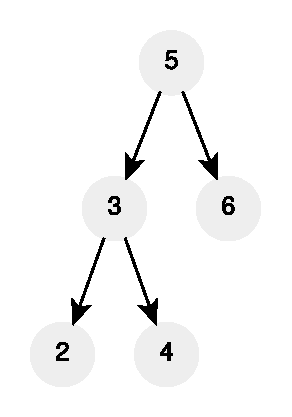
\includegraphics[width=\textwidth]{sources/kth_smallest_in_sorted_matrix/images/example1}
%	\caption[Sample short cpation]{Sample Caption}.
%	\label{fig:kth_smallest_in_sorted_matrix:example1}
%\end{figure}

\chapter{$k^{th}$ smallest element in a sorted matrix}
\label{ch:kth_smallest_in_sorted_matrix}
\section*{Introduction}
\begin{wraptable}{r}{4.5cm}
	\centering
	\begin{framed}  
	\begin{tabular}{|c|c|c|}
	\hline
	1  & 5  & 9  \\ \hline
	10 & 12 & 13 \\ \hline
	12 & 13 & 15 \\ \hline
\end{tabular}%
\caption{Tabular representation of Example \ref{example:kth_smallest_in_sorted_matrix:example1}}
\label{tab:kth_smallest_in_sorted_matrix:example1}
\end{framed}
\end{wraptable} 

One of the most common tool in computer science and engineering in general are rectangular grids of number also known as matrices\footnote{Matrices however are not stored in memory as grids. Computer memory is linear (think of it as a linear array) and therefore matrices must be mapped into it in some way. Turns out there is not only a single way of performing such a mapping, with the most common ones being \textit{row-major} and \textit{column-major}. The row-major stores each rows one after the other contiguously in memory  while column-major does the same but with columns. The matrix in Example \ref{example:kth_smallest_in_sorted_matrix:exercice1} would be stored as $\{\underbrace{1,5,9}_{\text{row 0}},\underbrace{10,12,13}_{\text{row 1}},\underbrace{12,13,15}_{\text{row 2}}\}$ in a row-major mapping and as $\{\underbrace{1,10,12}_{\text{col 0}},\underbrace{5,12,13}_{\text{col 1}},\underbrace{9,13,15}_{\text{col 2}}\}$as column-major}. The data they  contain can represent many things, from mathematical set of linear equations to algorithm for compression of images and videos or graphs.

In this chapter we are not going to worry about all of those super complex application of matrices and instead we will focus on a much simpler problem on a class of matrices of integers with the property of having rows and columns sorted. The task we need to perform on such a matrix is one that easily explained: we have to find the the $k^{th}$ smallest number among \textbf{all} values in the matrix.
This is one of such problem for which we will be able to find a working solution straigh-away, but coming up with a more time and space solution is way more complicated. 

On top of that, the naive solution different conceptually  quite a bit from the faster ones and that further complicates the solution process, especially during an interview. Most of us, once the naive solution is found, are will be naturally driven towards optimizing it, rather than trying to think about a radically different way to approach the problem.



\section{Problem statement}
\begin{exercise}
\label{example:kth_smallest_in_sorted_matrix:exercice1}
Write a function that, given an square matrix $M$ of size $n$  where each of individual row and column is sorted in ascending order and an integer $1 \leq k \leq n^2$
returns the $k^{th}$ smallest element in $M$.


You can assume the elements of $M$ to be always in the range $[0,n^2]$.

	%example1
	\begin{example}
		\label{example:kth_smallest_in_sorted_matrix:example1}
		\hfill \\
		Given $M=\{\{1,5,9\},\{10,12,13\},\{12,13,15\}\}$ (as shown in Table \ref{}) and $k=8$ the function returns $13$. See table
	\end{example}
\end{exercise}




\section{Clarification Questions}

\begin{QandA}
	\item Can we assume the input to be always valid i.e. having rows and column sorted?
	\begin{answered}
		\textit{Yes, there is no need to do input validation.}
	\end{answered}
	
	
\end{QandA}

\section{Discussion}
\label{kth_smallest_in_sorted_matrix:sec:discussion}


\subsection{Brute-force}
\label{kth_smallest_in_sorted_matrix:sec:bruteforce}

\lstinputlisting[language=c++, caption={Naive brute-force solution.},label=list:kth_smallest_in_sorted_matrix]{sources/kth_smallest_in_sorted_matrix/kth_smallest_in_sorted_matrix_solution1.cpp}

\subsection{Brute-force constant space}
\label{kth_smallest_in_sorted_matrix:sec:bruteforce_constant_space}

\lstinputlisting[language=c++, caption={Brute-force solution using constnat space.},label=list:kth_smallest_in_sorted_matrix]{sources/kth_smallest_in_sorted_matrix/kth_smallest_in_sorted_matrix_solution2.cpp}


\subsection{Binary Search}
\label{kth_smallest_in_sorted_matrix:sec:binarysearch}

\lstinputlisting[language=c++, caption={Solution using binary search.},label=list:kth_smallest_in_sorted_matrix]{sources/kth_smallest_in_sorted_matrix/kth_smallest_in_sorted_matrix_solution3.cpp}
